%---------------------------------------------------------------------
% This file provides a skeleton UCL DIS CDT report.
% \pdfinclusioncopyfonts=1
% This command may be needed in order to get \ell in PDF plots to appear. Found in
% https://tex.stackexchange.com/questions/322010/pdflatex-glyph-undefined-symbols-disappear-from-included-pdf
%---------------------------------------------------------------------
% Specify where LaTeX style files can be found.
\newcommand*{\DISCDTLATEXPATH}{latex/}
% Use this variant if the files are in a central location, e.g. $HOME/texmf.
%---------------------------------------------------------------------

\documentclass[NOTE, disdraft=true, UKenglish]{\DISCDTLATEXPATH UCLCDTDISdoc}
% The language of the document must be set: usually UKenglish or USenglish.
% british and american also work!
% Commonly used options:
%  cdtdraft=true|false   This document is a UCL CDT DIS draft.
%  paper=a4|letter       Set paper size to A4 (default) or letter.

%--------------------------------------------------------------------- 
% Add you own definitions here (file dis-gp-defs.sty).
%\usepackage{dis-gp-defs}
%---------------------------------------------------------------------


%--------------------------------------------------------------------- 
% Files with references for use with biblatex.
% Note that biber gives an error if it finds empty bib files.
\usepackage{biblatex} % uncomment if use addbibresource command
\addbibresource{template/PNET_project.bib}
%--------------------------------------------------------------------- 

% Paths for figures - do not forget the / at the end of the directory name.
\graphicspath{{logos/}{figures/}}


%---------------------------------------------------------------------
% Generic document information
%---------------------------------------------------------------------
% Title, abstract and document 
%-------------------------------------------------------------------------
% This file contains the title, author and abstract.
% It also contains all relevant document numbers if needed.
%-------------------------------------------------------------------------

% Partner Logo
% put the name of the logo image file found in graphics path
\DISPartnerLogo{logos/UCL_purple.png}


% Title
\DISTitle{Improving radiosensitivity predictions of brain cells using a biologically informed neural network}

% Draft version:
% If given, adds draft version on front page, a 'DRAFT' box on top of each other page, 
% and line numbers.
% Comment or remove in final version.
\DISVersion{0}

% Abstract - % directly after { is important for correct indentation
\DISAbstract{%
  One of the current most effective treatments for brain tumor's is radiotherapy. However, this has the side-effect of damaging healthy cells with potentially severe consequences. Improvements in radiotherapy treatment such as proton therapy allow a more spatially localized treatment. However, the sensitivity of different cell types to radioactivity is not currently well modeled. We present a method for predicting the radio-sensitivity of a cell based on its genetic content using a biologically informed neural network. We compare the use of different data features for training this model, different network architecture and develop a procedure for transfer learning, where drug response data is incorporated into the model training. We compare the model performance using a cross-validation procedure ensuring unbiased performance estimates with faithful uncertainty estimates. We find ...
}


% Authors and list of contributors to the analysis
\usepackage{authblk}
\author[a]{Toby Dixon}
\author[a]{Dakshesh Kololgi}
\author[b]{Jason Ran}

\affil[a]{University College London}


% DIS reference code if ever used
\DISRefCode{UCLCDTDIS-2024-XX}

% Author and title for the PDF file
\hypersetup{pdftitle={UCL CDT DIS Document},pdfauthor={The UCL CDT DIS}}

%---------------------------------------------------------------------
% Content
%---------------------------------------------------------------------
\begin{document}

\maketitle

\tableofcontents

\clearpage


%---------------------------------------------------------------------
\newpage
%---------------------------------------------------------------------

\newpage
%---------------------------------------------------------------------
\section{Introduction}
\label{sec:introduction}
Cancer is one of the largest causes of mortality in developed countries. This has led to intensive research into cancer treatments. One of the most promising is radiotherapy, in this treatment malignant tumors are treated with ionizing radiation (typically X-rays). However, these treatments still induce a significant amount of damage to healthy cells which can have severe effects. Developments in radiotherapy such as proton beam therapy \cite{proton_beam} allow for more spatially targeted treatments based on a patient's particular gene profile. This opens up the possibility of optimizing treatments to avoid regions expected to have high radiation sensitivity. Alongside such developments, advancements in gene sequencing technology and the availability of computational resources have staged genomics as an ideal problem for machine learning and artificial intelligence (AI) \cite{machine learning genomics}. In particular, \textit{Deep Learning} has the ability to create highly non-linear models which can make use of large feature spaces, which makes it a leading predictive model in genomics for accuracy, especially for \textit{sequence - to - activity} models. However, an emerging interest in such Deep Learning research has been model explainability, as these models are able to learn millions of model parameters to form predictions with none to little insight into how the prediction is made. This causes a problem in medical fields where often the understanding the causes and effects of processes are equally important. This problem is exacerbated by low data settings, where a large number of features are available for each data sample but only a small sum of samples are available, which can easily lead to over-fitting. At the current time, a lack of cells with both genetic and radiation sensitivity data available presents this exact issue. 

%%%In addition, developments in genetic sequencing mean that an increasing amount of genetic information is available to base radio-sensitivity predictions on. 
\\ \indent 
Predicting radio-sensitivity based on genetic data has been investigated using some classical approaches such as least squares regression \cite{SCOTT2017202}. In addition, machine learning methods could be employed as in \cite{speers2015development}. In general, these methods require heavy regularization due to the small available datasets.
\\ \indent  In this work we develop a radio-sensitivity predictor using a biologically informed neural network (BNN) \cite{review,review_2}. This type of model consists of a sparse neural network where the connections represent known biological processes, which are compiled in genetic databases \cite{reactome,go_1,go_2}. This has the advantage that the number of fitted parameters is much smaller, preventing over-fitting and the outputs of the model can be interpreted potentially leading to biological insights.
\\ \indent 
For this work, we use genomic data as predictors. This type of information is contained within a cell and enables its growth and reproduction. There are various sources of cancer cells used in medical research. These include patient-derived tumour xenografts (PDXs) - created by growing human tumour tissue in immunodeficient animal hosts \cite{NCBI}, which allows some physiological processes to take place when investigating human tumour cells. Another pre-clinical setting for human cell research are from \textit{cell lines}, which are human derived cells, which are in vitro cell populations. Cell lines have the advantage of being cost effective, providing a basis for reproducible results, and removes ethical concerns of human/animal tests. For an individual human, all their healthy cells have the same genetic foundation, characterised by their \textit{DNA} (deoxyribonucleic acid). DNA is a long double stranded helical molecule made of 4 nucleobases. Different sections of the DNA refer to different genes, which together with RNA (ribonucleic acid), allow for protein synthesis and other cell functions. Humans have approximately 20000 to 25000 genes \cite{Cleveland}. We focus on 3 genetic features; gene expression, copy number violation, and mutations. 
\\ \indent 
The model we will use called P-NET\cite{elmarakeby_biologically_2021}, was developed for the classification of prostate cancer cells. This model has been adapted for radio-sensitivity predictions \cite{cosmin_thesis}. In addition, we have explored applying transfer learning \cite{transfer} to radio-sensitivity predictions. In the P-NET setting, transfer learning aims to make use of similarities between the underlying cellular processes of drug and radiation response. This requires a model to be trained using information from drug response data, which is more readily available.
\\ \indent 
This report describes a systematic comparison of P-NET used for radiation predictions using different data types and network architectures. 
In \ref{sec:data} we describe the genetic data used for this study, in \ref{sec:method} we describe in more detail the model and our framework for model comparisons. Finally, in section \ref{sec:results} we describe the results. The outlook for future studies is described in \ref{sec:conclusion}.
 
%\input{introduction}
%---------------------------------------------------------------------
\section{Data}
\label{sec:data}


\begin{figure}
    \centering
    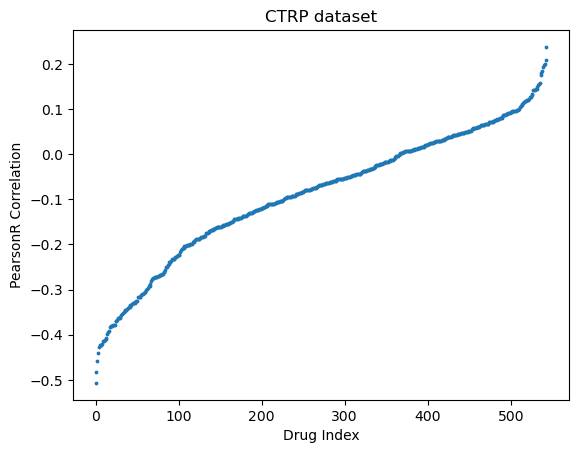
\includegraphics[width=9cm]{Figures/CTRP_correlation.png}
    \caption{CTRP correlation}
    \label{CTRP correlation}
\end{figure}
%We use data from the Cancer Cell Line Encyclopedia (CCLE) dataset \cite{ccle}.

\\ \indent 
This dataset contains measurements \cite{yard} of the radio-sensitivity of 511 cell lines along with their genetic data.
The radio-sensitivity is characterized by the area under the dose-response curve (AUC). 
This is a relatively expensive measure requiring irradiation of cells with known doses of radiation. This limits the size of the available dataset. 


{   \color{red}
Still to include:
\begin{itemize}
\item breif description of basic interaction between DNA, RNA and protein synthesis?
\item explanation of datasets needed for transfer learning
\item explanation of PharmacoGx and RadioGx packages (Manem et al) and how transfer learning datasets are obtained (taking cell lines with gene expression data etc.)
\end{itemize}}

\section{Methods}
\label{sec:method}
For this work, we employ a biologically informed neural network to predict the radio-sensitivity. This is based on our adaptation of P-NET \cite{cosmin_thesis}. A typical dense neural network has millions of connections, and thus weights to tune. This can easily lead to over-fitting where the model predicts well on the training dataset but not on unseen data. A solution to this is to encode some prior knowledge into the model's architecture. In this way, we create a sparse network where the connections represent known biological pathways.

\subsection{Network architecture}
P-NET is a feed-forward Biologically Informed Neural Network originally developed to classify prostate cancer tumours into being either primary or metastatic types. P-NET consists of six layers arranged such that the constituent neurons encode the hierarchical manner of the Reactome or Gene Ontology bio-informatics databases. Each successive layer encodes increasingly more complex biological processes. This was implemented by selectively connecting neurons between layers depending on the hierarchies in Reactome or Gene Ontology.

This work significantly re-structured P-NET to enable connections between layers to be informed by Gene Ontology in addition to Reactome. We draw from Kuenzi et al.'s implementation of the DrugCell Deep Learning model that, in analogy with P-NET, utilises Gene Ontology for cancer cell drug sensitivity prediction \cite{kuenzi_predicting_2020}.

\begin{figure}
    \centering
    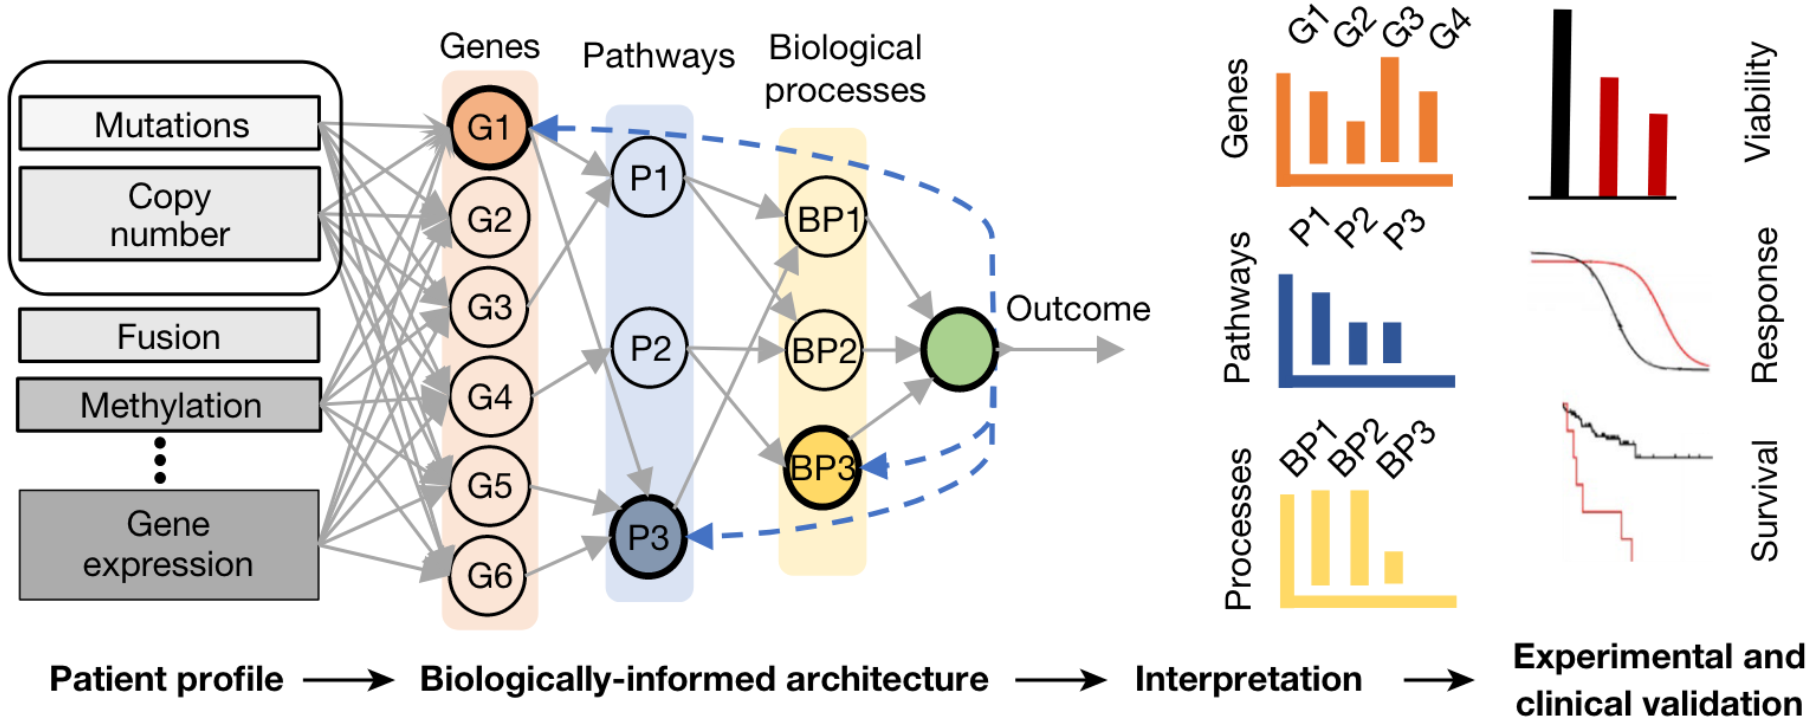
\includegraphics[width=\linewidth]{Figures/pnet_architecture.png}
    \caption{Architecture of the original P-NET neural network \cite{elmarakeby_biologically_2021} informed by the Reactome database. The number of nodes in the first layer corresponds to the number of genes in the Reactome database. These genes code for proteins, pathways and biological processes.}
    \label{fig:1}
\end{figure}

While the default first layer, which represents genes contains 14657 neurons, the biologically informed nature of P-NET has a reduced training speed over a fully connected network as the reduced number of connections results in fine-tuning of a gene set by only considering sub-graphs of the original network without entropy loss. The biologically informed nature of P-NET has inherent interpretability because each neuron is either a gene, pathway or process, so, predictions could be interpreted as the activation of particular biological mechanisms.

\begin{figure}
    \centering
    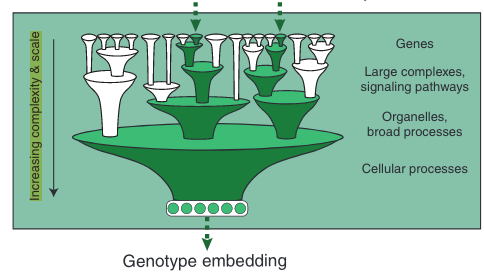
\includegraphics[width=\linewidth]{Figures/drugcell_architecture.png}
    \caption{DrugCell's \cite{kuenzi_predicting_2020} architecture, it is analogous to Reactome but the genes, biological processes and pathways are constructed independently and may not overlap.}
    \label{fig:2}
\end{figure}

We implemented the variant of P-NET informed by Gene Ontology through significantly restructuring the P-NET codebase. The DrugCell code provided by Kuenzi et al. \cite{kuenzi_predicting_2020} was the source of the Gene Ontology gene-pathway hierarchy and was copied into the same directory as the Reactome hierarchy. Then additional functions were created within a new file, $\mathtt{pathway\_encoder.py}$, that utilised a class-based code structure to eliminate redundancy. This was a crucial element of our adaptation of P-NET because it facilitated us to test Reactome and Gene Ontology with a fixed procedure of performance evaluation and hyperparameter optimisation.

\subsection{Loss function}
Each of the 6 layers of the network can be used to predict the radio-sensitivity. To prevent each layer from inheriting features from its parent \cite{cosmin_thesis}, P-NET uses a loss function built by combining the predictions from each of the 6 layers using a vector of loss weights.  We chose the mean squared error as our loss function.
We kept this at the default value for P-NET shown in Table \ref{tab:hyperpars}.
\subsection{Regularization}
Despite the sparse network, the model is still prone to over-fitting. To prevent this we employ $\mathtt{L2}$ regularization. This consists of adding a penalty term to the loss function:
\begin{equation}
    L_{L2} = \lambda \times \sum ||w||^2,
\end{equation}
for all the model weights $w$. This term will push the model towards smaller weights (or thus a simpler model). This term is characterised by the regularisation parameter $\lambda$, too small a value will lead to model overfitting, while too large can cause the weights to diverge to 0. In this case, the model will not predict any variability and instead predict for all outputs the mean of the training data.
\subsection{Early stopping}
We employ early stopping \cite{keras-docs} when training the model to further prevent over-fitting and improve training speed. This prevents very continuing training for many epochs, which while improving the loss function may decrease the validation data loss function. We employ early stopping using a patience of 5, this means that if the validation loss function increases for the patience number of consecutive epochs the training is halted and the weights with the lowest validation loss are used. We tested increasing the patience value but this had negligible effects.
It should be noted that this procedure could potentially lead to a biased validation performance estimate. However, our final performance is quoted on test and not validation data.
\subsection{Transfer learning}
As previously mentioned in \ref{sec:introduction}, the difficulties in obtaining radio-sensitivity data for human tumour cell lines has provided us with a relatively small dataset of 511 cell lines from the Cleveland dataset. The sparsity P-NET (order 10**5 trainable parameters) has demonstrated improved performance when compared to fully dense networks (order 10**7 trainable parameters), particularly in low data settings by avoiding over-fitting \cite{elmarakeby_biologically_2021}. 

Clearly then, the supplementation of additional information to the Cleveland set may further improve generalisation of the P-NET model. This idea forms the basis of \textit{transfer learning}, where knowledge from related fields can be used to inform machine learning models trained on either field. In the context of this work, our aim is to predict radio-sensitivity, and we hope to use data from drug sensitivity to perform transfer learning. For certain drugs, the underlying cellular processes that cause cell death and proliferation will have similarities to radiation, thereby being more suited for transfer learning. Luckily, databases related to drug response are somewhat more extensive than that of radiation, as discussed in \ref{sec:data}. As seen in Figure \ref{fig:3}, transfer learning assumes that the lowest level features and connections (relations between individual genes) remain somewhat consistent from drug response to radiation response. By training a network on drug response and transferring (and freezing) the lowest layers, the model trained radiation response can be fitted using fewer trainable parameters with hopes of improving performance and reducing over-fitting.

{   \color{red}
Include:
\begin{itemize}
\item Description of transfer learning procedure (relating to CV and hyperparameter tuning)
\item Discussion of mechanisms of action and their expected effect
\end{itemize}}

\begin{figure}
    \centering
    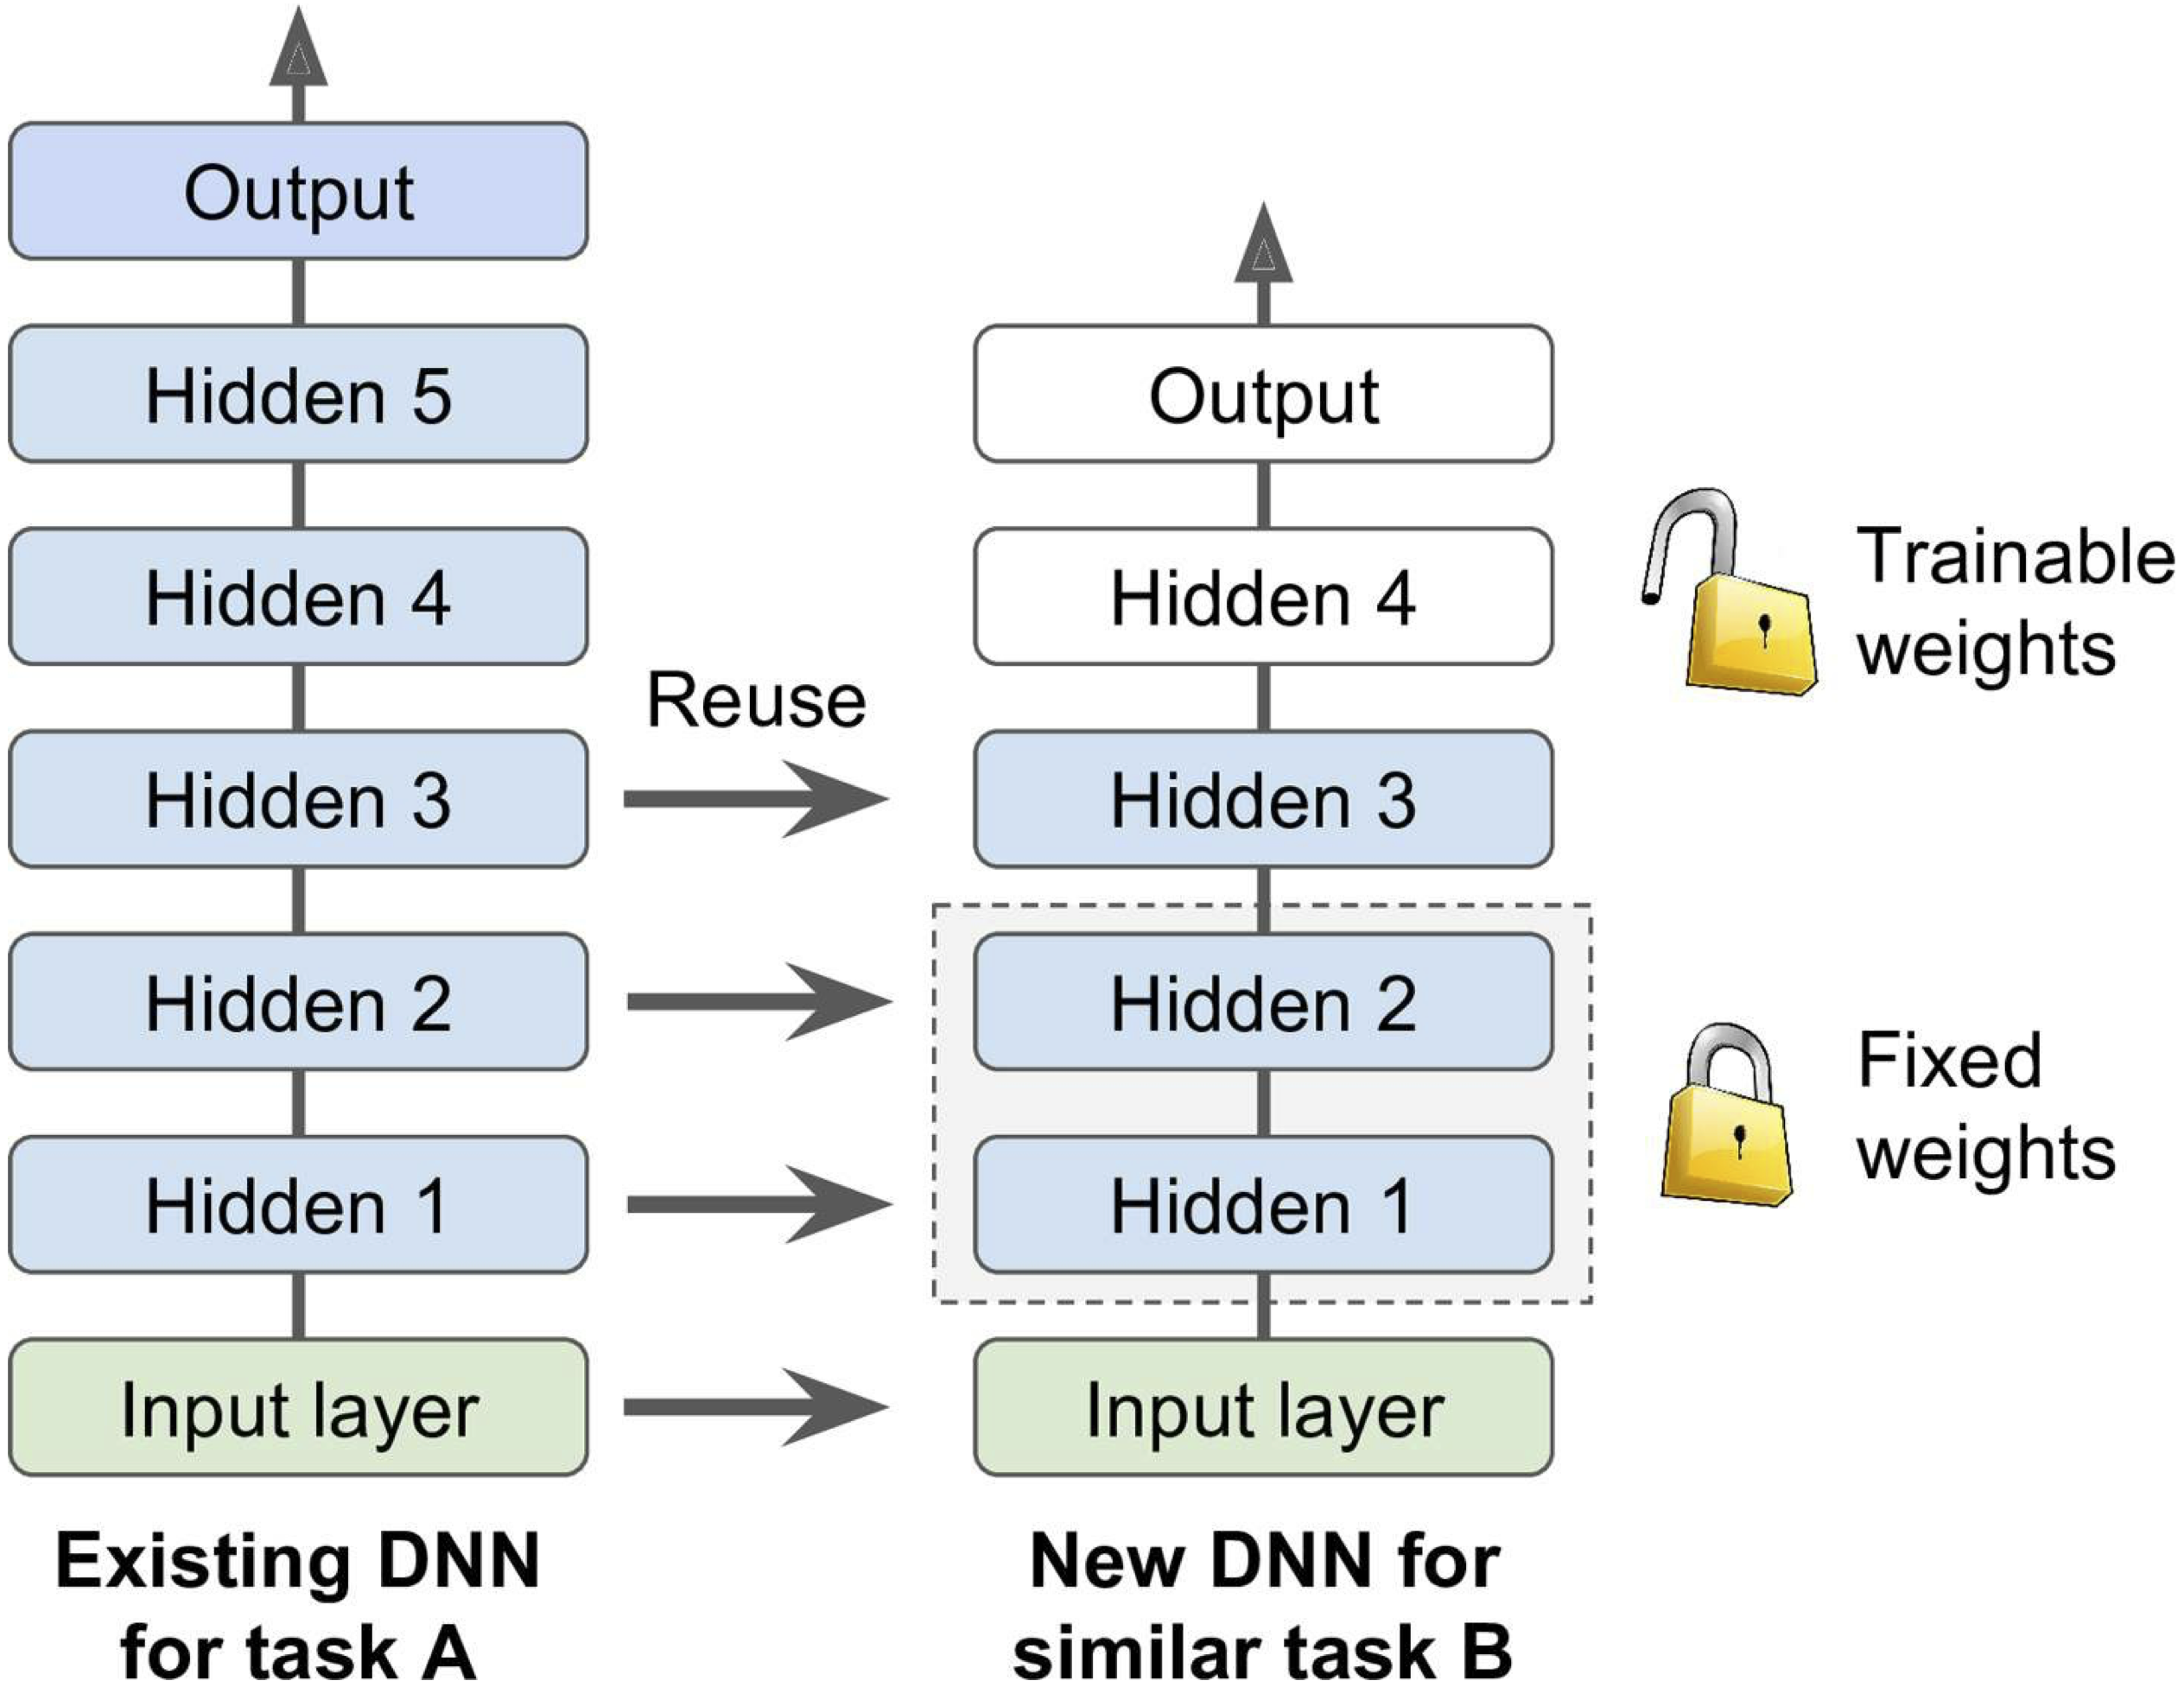
\includegraphics[width=6cm]{Figures/transfer_learning.png}
    \caption{Transfer learning procedure in neural networks \cite{McEwann lecture}}
    \label{fig:3}
\end{figure}
\subsection{Cross-validation and hyper-parameter tuning}
Due to the very small available datasets we found the performance of a given model can vary significantly based on the test splitting of the data. In addition, the performance can vary based on the random seeds used in the stochastic minimisation of the loss function. We also found that the performance can depend significantly on model hyper-parameters. If these are tuned to optimise the performance on a particular test splitting of the data this will result in an overly optimistic estimate of the performance when trained on unseen data.
\\ \indent To account for this we have developed a cross-validation procedure. This is used both to tune hyper-parameters and to make an unbiased estimate the model performance with a faithful uncertainty estimate. This procedure allows a fair comparison of different models.
\\ \indent We employ a procedure of nested-random-cross-validation \cite{cross_validate}.
A set of randomly chosen test datasets  are selected. In each case the remaining data is used to tune the model hyper-parameters. For this we use a grid search with random-cross validation. For every hyper-parameter set the data is is partitioned into a validation and a training set. The model training is run using the validation set to decide the early stopping of the training and to estimate the performance. This is then repeated a number of times to obtain an estimate of the mean performance and uncertainty for this hyper-parameter set. The hyper-parameter set with the best model performance are then used to train the model, with the performance judged on the test dataset. The distribution of this testing performance give an unbiased estimate of the model performance, with a reliable uncertainty estimate. This procedure is very computationally intensive and has been implemented using batch job submission in parallel on the Myriad cluster at UCL \cite{myriad}.
\\ \indent There are a number of hyper-parameters potentially affecting the model performance. For example the learning rate of the gradient descent and learning rate schedule, L2 regularisation parameters, drop-out parameters etc (see more details in the previous section). 
These hyper-parameters can broadly be divided into two classes, those which control the minimisation of the loss function and those which add some terms / modify it to prevent over-fitting. We found most of the hyper-parameters are correlated so focused on two for a optimisation, the learning rate and the regularisation parameter which are tuned using a grid search.  
\\ \indent Other model hyper-parameters are not formally optimized. To prevent bias these were set to reasonable values based on the $\mathtt{scikit-learn}$ and tensor-flow documentation and some initial tests on a single train / validation set. 
The choice of parameters is specified in Table \ref{tab:hyperpars}.
\begin{table}[]
    \centering
    \begin{tabular}{c|c}
       Hyperparameter  &  Value \\ \hline
       Regularisation parameter & Optimised - see text \\
       Learning rate  & Optimised - see text \\
      batch size  & 50 \\
      Early stopping patience &  5 \\
     Maximum number of epochs &  50 \\
     Optimiser &   Adam \\
     Loss weights &  $[1, 15, 20, 54, 240, 380]$ 
    \end{tabular}
    \caption{The various hyperparameters used in training P-NET for radiation sensitivity.}
    \label{tab:hyperpars}
\end{table}
\\ \indent To asses model performance we compute the $R^2$ score defined as \cite{scikit-learn-docs}:
\begin{equation}
    R^2 = 1-\frac{\sum (y_i - \hat{y}_i)^2}{\sum_i (y_i - \bar{y})^2},
\end{equation}
where $y_i$ the value for data-point $i$, $\hat{y}_i$ is the associated prediction, while $\bar{y}$ is the mean of $y$. This gives a measure of the amount of variance in the outputs explained by the model.
%\input{method}

%---------------------------------------------------------------------


\section{Results}
\label{sec:results}
\\
We use a biologically informed neural network based on P-NET \cite{elmarakeby_biologically_2021} to predict the radiation sensitivity of 511 cell lines. 
We performed a systematic comparison of P-NET applied to radio-sensitivity predictions using both the Reactome \cite{reactome} and Gene ontology \cite{go_1,go_2} databases and gene expression, copy number variation and mutation data separately. 
\subsection{Reactome network}
First we present results for the model trained using the Reactome network architecture. In \cite{cosmin_thesis}, a similar model was trained using gene expression and copy number violation data. This study used a fix train/test/validation split and hyper-parameter tuning was performed manually. 
We reproduce this study using the same data splitting, but with optimisation of the learning rate and regularisation. 
\\ \indent We observed a large variation in the validation and test performance when changing the random seed used in the batch gradient descent.
This large observed variability is related to the small size of the dataset, along with large number of features. This leads to a large number of local minima in the loss function. 
\\ \indent We optimise the learning rate and regularisation parameter for this dataset. A grid search is performed in the range of $\log{\alpha}\in [-3,0]$ with 20 steps and $\log{\lambda}\in [-8,0]$ with 20 steps. For each hyper-parameter set the training is run 50 times.
In Fig. \ref{fig:example_scan} we show the mean and standard deviation of the validation data $R^2$ distribution for each hyper-parameter set. The best value is found to be XX, and YY, which leads to average performance of:
\begin{equation}
    R^2 (\mathrm{train})&=X\pm Y \ \%, \ \       R^2 (\mathrm{validate})&=X\pm Y \ \%, \ \
    R^2 (\mathrm{test})&=X\pm Y \ \%. 
\end{equation}
This estimate of the performance is likely biased and was only computed for a comparison with \cite{cosmin_thesis} where a value of 31 \% for test and 42\% for training data was obtained. These values are compatible given the large observed spread in the results.
An example of the training and test predictions are given in Fig. \ref{example_scatter}.
The distribution of $R^2$ and mean squared error (MSE) for the optimal hyper-parameters is shown in Fig. \ref{dist}.
\\ \indent 
We then repeat this optimisation procedure varying the validation split (as described earlier). In this case the optimal set of hyper-parameters are XXX and YYY leading to average performance of:
\begin{equation}
    R^2 (\mathrm{train})&=X\pm Y \ \%, \ \       R^2 (\mathrm{validate})&=X\pm Y \ \%, \ \
    R^2 (\mathrm{test})&=X\pm Y \ \%. 
\end{equation}
This performance is notably worse than that obtained on a single validation/ test dataset. This demonstrates the bias induced by tuning hyper-parameters to a single dataset and motivated the development of the nested-cross validation procedure described earlier. It should be noted that this performance estimate may also be biased.
\\ \indent We use the nested cross-validation procedure defined earlier to provide an unbiased estimate of the model performance. Due to the computational demands of this procedure a scan of 10 steps is used, with 10 validation splittings used per hyper-parameter set. This is then repeated for 10 test splittings of the data. Across these 10 random test splittings we observe performance of:
\begin{equation}
    R^2=X \pm Y.
\end{equation}
This indicates that P-NET trained using this data provides a relatively poor and very unstable prediction of radiation sensitivity. This motivated the development of the transfer learning algorithm described earlier.
\subsection{Gene Ontology network}
We repeat this procedure of using the Gene Ontology network again using Gene Expression data. The results of a single hyper-parameter scan are shown in Fig. \ref{fig:go}. The average performance is:
\begin{equation}
    R^2=X\pm Y.
\end{equation}
While this is notably worse than the performance from Reactome, it is likely some other hyper parameters of the model need to be adjusted for the Gene Ontology network architecture.
\subsection{Systematic comparison of data types and architecture}
We repeat the procedure defined above for each data type and for the Gene Ontology as well as Reactome network. The results are shown in Tab. \ref{tab:perf}. This represents the first systematic comparison with unbiased performance estimates including uncertainties of a biologically informed neural network applied to radiation prediction using different network architecture and data types.
\begin{table}[]
    \centering
 \caption{$R^2$ performance of P-NET obtained using nested random cross validation, for different network architecture and data types.}

    \begin{tabular}{c|c|c}
     Data Type    & Network & Test $R^2$  \\ \hline
     \\
     \\
     \\
     \\
     \\
         & 
    \end{tabular}
 
    \label{tab:perf}
\end{table}
\\

\subsection{Transfer learning}
Using the Reactome network, we train a transfer learning model on the 10 most correlating with at least 300 cell lines available.

{   \color{red}
Include:
\begin{itemize}
\item plots of individual drug sensitivity prediction performance (i.e. before transfer learning)
\item side - by - side plots scatter of P-NET with and with-out transfer learning
\item quantitative description of performances (with uncertainties)
\item comments on performance of each drugs in general - relating to mechanisms of action
\end{itemize}}

%\input{results}
%---------------------------------------------------------------------

\section{Discussion}
\label{sec:conclusion}
{   \color{red}
Include:
\begin{itemize}
\item rename to "Discussion"
\item relate back to introduction
\item Discussion of how this work builds upon the group's previous work (picked up from Cosmin's thesis)
\item discuss Cosmin's work to turn the code base into a Python package, and how our work fits into that
\item more sophisticated models to work on in the future (how can meta/multitask learning can be developed from our work)
\item how does this project fit into the wider work of the Dean lab (work from Felix, Amin etc.)
\item limitations and future work
\end{itemize}}
In this report we presented predictions of cell line radio-sensitivity using a biologically informed neural network trained on genetic data. We use an implementation of a BNN based on the P-NET architecture and code base. This has been significantly refactored to allow for systematic tuning of hyper parameters and nested-random-cross validation run on a high performance computing cluster and to include the Gene-Ontology network architecture. 
\\ \indent 
We performed a systematic comparison of different network architectures and multi-omic data types. This showed the model is moderately successfully in predicting radio-sensitivity with the best case being XXX which resulted in $R^2=Y$. In addition, we have investigated an improvement to this model using transfer learning of drug response data. We obtained promising results showing that the BNN is able to predict well the drug response in some cases and that this may improve the radio-sensitivity predictions.
\printbibliography
%\input{conclusion}
%---------------------------------------------------------------------

\end{document}
